\subsubsection{\stid{4.16} ALPINE} 


\paragraph{Overview} 

ECP ALPINE will deliver in situ visualization and analysis infrastructure to ECP Applications.  
%
ALPINE developers come from the ParaView~\cite{paraview1,paraview2} and VisIt~\cite{VisIt} teams and ALPINE solutions will deliver in situ functionality in those tools, as
well as ASCENT~\cite{ASCENT}, a new in situ solution that focuses on flyweight processing. 
%
The ALPINE team focuses on four major activities: 
\begin{enumerate}
        \setlength{\itemsep}{1pt}
        \setlength{\parskip}{0pt}
        \setlength{\parsep}{0pt}
\item Deliver Exascale visualization and analysis algorithms that will be critical for ECP Applications as the dominant analysis paradigm shifts from post hoc (post-processing) to in situ (processing data in a code as it is generated). 
\item Deliver an Exascale-capable infrastructure for the development of in situ algorithms and deployment into existing applications, libraries, and tools. 
\item Engage with ECP Applications to integrate our algorithms and infrastructure into their software. 
\item Engage with ECP Software Technologies to integrate their Exascale software into our infrastructure. 
\end{enumerate}


\paragraph{Key  Challenges}

Many high performance simulation codes are using post hoc processing, meaning they write data to disk and then visualize and analyze it afterwards. 
%
Given Exascale I/O constraints, in situ processing will be necessary. 
%
In situ data analysis and visualization selects, analyzes, reduces, and generates extracts from scientific simulation results during the simulation runs to overcome bandwidth and storage bottlenecks associated with writing out full simulation results to disk. 

The ALPINE team is addressing two problems related to Exascale processing --- (1) delivering infrastructure and (2) delivering in situ-appropriate algorithms.
%
For delivering infrastructure, the challenge is that our existing tools are not ready for Exascale.
%
In particular, we are concerned about achieving performance within simulation codes' time budgets, supporting many-core architectures, scaling to massive concurrency, and leveraging deep memory hierarchies.
%
For in situ-appropriate algorithms, the challenge is that our stakeholders need to be able to apply in situ processing effectively without a human being in the loop.
%
This means that we must have approaches to automate saving either the correct visualizations or the correct data extracts.


\paragraph{Solution Strategy}

A major strategy for our team is to leverage existing, successful software, ParaView and VisIt, including their recent developed in situ libraries Catalyst~\cite{Catalyst} and Libsim~\cite{LibSim}, and then to integrate and augment them with ALPINE capabilities to address the challenges of Exascale. 
%
Both software projects represent long-term DOE investments, and they are the two dominant software packages for large-scale visualization and analysis within the DOE Office of Science (SC) and the DOE National Nuclear Security Agency (NNSA). 
%
These two products will provide significant coverage of ECP Applications, and we can leverage their existing engagements to deliver ALPINE's algorithms and infrastructure. 
%
%Our development strategy consists of placing all new algorithms developed in a single code repository, and deploying this code in both
%ParaView and VisIt.
%
We are also developing another in situ library, ASCENT, with also utilizes this code repository; ASCENT is a ``flyweight'' solution,
meaning that it is focused on a streamlined API, minimal memory footprint, and small binary size.

In terms of specifics, our solution strategy is two-fold, in response to our two major challenges (infrastructure and algorithms).

For infrastructure, we have developed a layer on top of the VTK-m library for ALPINE algorithms.
%
This layer is where all ALPINE algorithms will be implemented, and it is deployed in ParaView, VisIt, and ASCENT.
%
This means that all development effort by ALPINE will be available in all of our tools.
%
Further, by leveraging VTK-m, we will be addressing issues with many-core architectures.
%
Figure~\ref{fig:alpine_infrastructure} illustrates our software strategy.

\begin{figure}[htb]
	\centering
	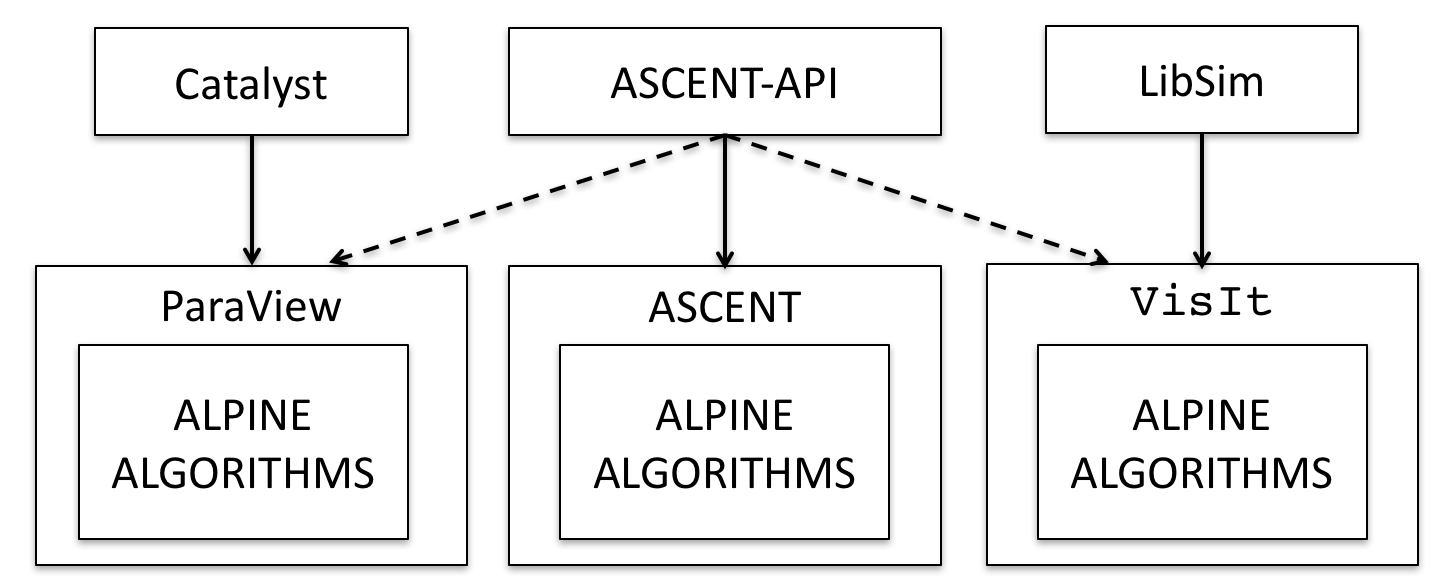
\includegraphics[width=3in]{projects/2.3.4-DataViz/2.3.4.16-ALPINE-ZFP/alpine_infrastructure.png}
	\caption{\label{fig:alpine_infrastructure}ALPINE's strategy for delivering and developing software.  We are making use of existing software (ParaView, VisIt), but making sure all new development is shared in all of our tools.  The dotted lines represent future work, specifically that the ASCENT API will work with ParaView and VisIt.}
\end{figure}

For automating in situ, we are pursuing four different algorithms:
\begin{itemize}
        \setlength{\itemsep}{1pt}
        \setlength{\parskip}{0pt}
        \setlength{\parsep}{0pt}
\item \textbf{Feature-based analysis} with moments to detect rotation-invariant patterns.  These patterns can then be used either to direct which features should be visualized or to direct which extracts should be saved.
\item \textbf{Lagrangian analysis} of vector flow allows more efficient and complete analysis and tracking of flow.  It is a method for saving vector field data with more higher accuracy and less storage than the traditional approach.
\item \textbf{Topological analysis} can be used to detect features in the data and steer visualizations.  For example, contour trees can identify the most significant isosurfaces in complex simulations and then the resulting visualizations can use these isosurfaces.
\item \textbf{Importance sampling} can be used to guide visualizations and extracts to the most important parts of the simulation.  Examples ranges from clustering similar data points within a region to identifying important time slices to save.
\end{itemize}




\paragraph{Recent Progress}

Again, we organize our recent progress around infrastructure and algorithms.

On the infrastructure side, we have completed the layer on top of VTK-m for ALPINE algorithms (Milestone STDA04-2, https://gitlab.kitware.com/vtk/vtk-m). 
%
We have stood up ASCENT, our flyweight in situ library, including defining its API (STDA04-1), making an initial release (STDA04-11), and making a production release (STDA04-30, https://github.com/Alpine-DAV/ascent).
Most recently, we integrated VTK-m into VisIt and ParaView and integrated our algorithms into our ALPINE infrastructure (STDA04-32, https://github.com/Alpine-DAV/vtk-h).

On the algorithms side, we have been researching and developing our four algorithms (STDA04-5).
%
In all cases, the progress is a combination of evaluating best approaches, and developing VTK-m based solutions that
can be deployed in our infrastructures.
%
Our topological analysis work resulted in some early successes.
%
With this work, there is now a VTK-m implementation, although it needs additional effort for distributed memory support.
%
The algorithm was applied to a WarpX simulation (STDA04-15), and used to automatically select isovalues in situ.
%
Figure~\ref{fig:alpine_topology} compares the traditional approach with our enhanced version.
%
With our latest milestone (STDA04-33), we are demonstrating each of our four algorithms with ECP Applications --- running an example of moment detection on MFIX data, demonstrating sampling performance for an MFIX particle data set, running in situ topological analysis for WarpX, and applying Lagrangian methods to Nyx data.

\begin{figure}[htb]
	\centering
	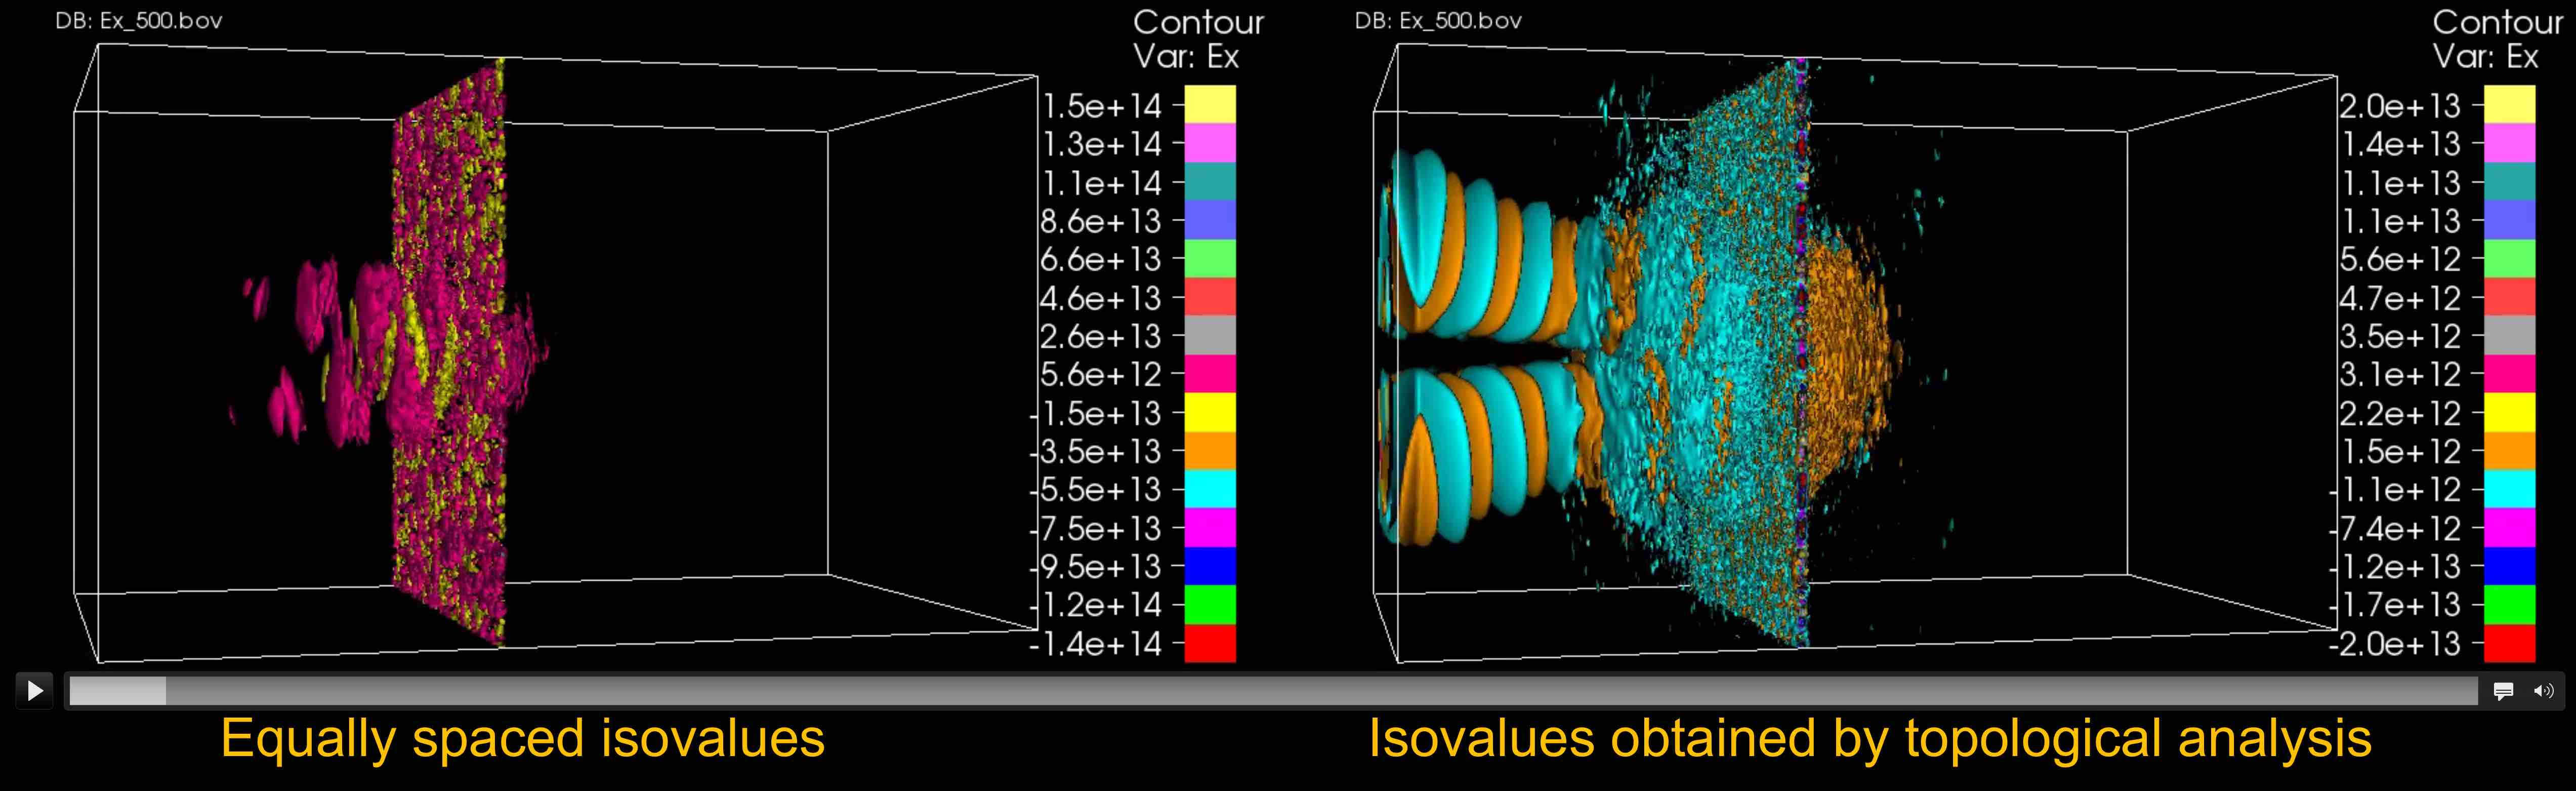
\includegraphics[width=4in]{projects/2.3.4-DataViz/2.3.4.16-ALPINE-ZFP/alpine_topology}
	\caption{\label{fig:alpine_topology}In situ visualizations taken from WarpX using VisIt.  At left, equally spaced isovalues in an ion accelerator simulation. At right, our method chooses isovalues using topological analysis to more fully represent complex behavior in the data.}
\end{figure}


\paragraph{Next Steps}

We have three milestones remaining, one for algorithms, one for infrastructure, and one for outreach with ECP Applications.
\begin{itemize}
        \setlength{\itemsep}{1pt}
        \setlength{\parskip}{0pt}
        \setlength{\parsep}{0pt}
\item For infrastructre, our next major activity is to fully integrate ALPINE infrastructure into ParaView and VisIt (STDA04-36).
\item For algorithms, our next major activity is optimization, refinement, hardening, and extension of the developed in situ algorithms, including in situ demonstrations (STDA04-37).
\item For outreach, we will do an end-to-end demonstration of automatic data selection, automatic data reduction, and extract processing algorithms using  our in situ infrastructure for ECP Applications (STDA04-38).
\end{itemize}
